\subsection{Alumno curso académico}

  \paragraph{}Se procede a crear el alumno curso académico, en este caso, el
  alumno recientemente creado, en el curso académico 2010. Para ello, se
  realizará la creación de un alumno curso académico, tal y como se describió en
  el capítulo \ref{addAlumnoCA}, \textit{Añadir alumno curso académico}.

  \paragraph{}Una vez que aparezca el formulario de creación, se debe introducir
  el curso académico en dicho formulario, con lo que la pantalla quedaría tal y
  como refleja la figura \ref{ejemploAddAlumnoCA}.

  \begin{figure}[!ht]
    \begin{center}
      \fbox{
      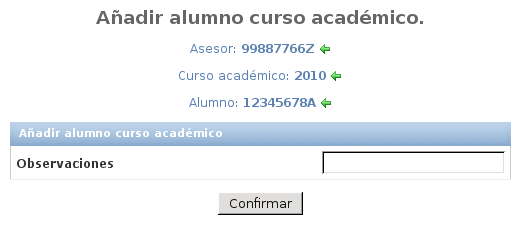
\includegraphics[scale=0.55]{5.Ejemplos_Practicos/5.3.IntroduccionDatos/5.3.9.AlumnoCA/add_alumnoCA.png}
      }
      \caption{Creación de \textit{Alumno curso académico} de ejemplo.}
      \label{ejemploAddAlumnoCA}
    \end{center}
  \end{figure}

  \paragraph{}Una vez rellenado el formulario, se pulsará el botón
  \textit{Confirmar}, el cual se puede ver en la figura
  \ref{capturaBotonConfirmar}. Si el formulario rellenado es válido, y no tiene
  errores, se creará el nuevo elemento en el sistema. En caso de contener
  información no válida, un mensaje de error aparecerá indicando los campos
  del formulario que no han pasado la validación, los cuales habrá que modificar
  para introducir correctamente el elemento en el sistema.
